\documentclass[11pt,a4paper]{article}

% --- Packages ---
\usepackage[utf8]{inputenc}
\usepackage[T1]{fontenc}
\usepackage{lmodern}
\usepackage[margin=0.8in, top=1.2in]{geometry}
\usepackage{xcolor}
\usepackage{titlesec}
\usepackage{hyperref}
\usepackage{enumitem}
\usepackage{booktabs}
\usepackage{amsmath}
\usepackage{amssymb}
\usepackage{graphicx}
\usepackage{fancyhdr}
\usepackage{tcolorbox}
\usepackage{lastpage}
\usepackage{tikz}
\usepackage{pgfplots}
\usepackage{multicol}
\usepackage{wrapfig}
\usepackage{float}
\usepackage{array}
\usepackage{colortbl}
\usepackage{soul}

% --- Custom Colors ---
\definecolor{mn-navy}{RGB}{10, 25, 47}
\definecolor{mn-blue}{RGB}{0, 119, 181}
\definecolor{mn-slate}{RGB}{73, 94, 117}
\definecolor{mn-light}{RGB}{240, 244, 248}
\definecolor{mn-accent}{RGB}{255, 107, 53}
\definecolor{mn-success}{RGB}{76, 175, 80}
\definecolor{mn-warning}{RGB}{255, 152, 0}
\definecolor{mn-error}{RGB}{244, 67, 54}

% --- Header & Footer with Rounded Box ---
\pagestyle{fancy}
\fancyhf{}
\lhead{\textcolor{mn-slate}{\small \textbf{MarketNerve Product Blueprint}}}
\rhead{\textcolor{mn-slate}{\small Chanikya Nelapatla}}
\cfoot{\small \textcolor{mn-slate}{Page \thepage\ of \pageref{LastPage}}}
\renewcommand{\headrulewidth}{1pt}
\renewcommand{\headrule}{\color{mn-blue}\hrule width\headwidth height\headrulewidth \vskip-\headrulewidth}

% --- Section Styling with Enhanced Visual Hierarchy ---
\titleformat{\section}
{\color{mn-navy}\normalfont\Large\bfseries}
{\colorbox{mn-light}{\textcolor{mn-blue}{\thesection}}}
{0.8em}
{}
[{\tikz[remember picture, overlay]{\draw[line width=2pt, color=mn-blue] (0,0) -- (\linewidth,0);}}]

\titleformat{\subsection}
{\color{mn-blue}\normalfont\large\bfseries}
{\color{mn-blue}\thesubsection}
{1em}
{}

\titleformat{\subsubsection}
{\color{mn-slate}\normalfont\normalsize\bfseries}
{\color{mn-slate}\thesubsubsection}
{0.8em}
{}

\titlespacing{\section}{0pt}{12pt plus 4pt minus 2pt}{8pt plus 2pt minus 2pt}
\titlespacing{\subsection}{0pt}{10pt plus 3pt minus 2pt}{6pt plus 1pt minus 1pt}

% --- Custom Commands ---
\newcommand{\feature}[1]{\small\textcolor{mn-success}{\facheck\ #1}}
\newcommand{\highlight}[1]{\colorbox{mn-light}{\textcolor{mn-navy}{#1}}}
\newcommand{\riskbox}[1]{\tcbox[colback=mn-error!10, colframe=mn-error, arc=1mm]{#1}}
\newcommand{\infobox}[1]{\tcbox[colback=mn-light, colframe=mn-blue, arc=1mm]{#1}}

% --- Document Start ---
\begin{document}

% --- Enhanced Cover Page ---
\thispagestyle{empty}
\begin{titlepage}
    \centering
    
    % Decorative top bar
    {\color{mn-navy}\hrule height 0.3cm\relax}
    
    \vspace*{3.5cm}
    
    % Logo placeholder
    \includegraphics[width=3cm]{logo.png}
    
    \par \vspace{1.5cm}
    
    {\Huge \bfseries \color{mn-navy} MarketNerve} \par
    \vspace{0.5cm}
    {\Large \color{mn-blue} Product Blueprint \& Architectural Framework} \par
    \vspace{0.3cm}
    {\small \color{mn-slate} Decision Intelligence System for Indian Retail Investors}
    
    \vspace{2.5cm}
    
    % Information Box
    \begin{tcolorbox}[colback=mn-light, colframe=mn-navy, width=\textwidth, arc=3mm, boxsep=12pt, left=15pt, right=15pt]
        \begin{center}
            \textbf{\color{mn-navy}\Large ET Gen AI Hackathon} \par
            \vspace{0.8cm}
            {\color{mn-slate}\begin{tabular}{@{}ll@{}}
                \textbf{Prepared by:} & Chanikya Nelapatla \\
                \textbf{Date:} & \today \\
                \textbf{Version:} & 1.2 (Enterprise Grade)
            \end{tabular}}
        \end{center}
    \end{tcolorbox}
    
    \vfill
    
    % Subtitle box
    \begin{tcolorbox}[colback=mn-blue!5, colframe=mn-blue, width=\textwidth, arc=2mm]
        {\small \color{mn-slate}
        MarketNerve: An intelligence system that transforms fragmented market data into ranked opportunities, technical conviction signals, portfolio-aware reasoning, and narrative context with confidence scoring, statistical ranking, and evidence-first decision support for Indian retail investors.
        }
    \end{tcolorbox}
    
    \vspace{1.5cm}
    
\end{titlepage}

% --- Table of Contents ---
\newpage
\setcounter{page}{2}
{\color{mn-navy}\tableofcontents}
\newpage

% ===============================================
% SECTION 1: EXECUTIVE SUMMARY
% ===============================================
\section{Executive Summary}

MarketNerve is a \highlight{decision-intelligence operating layer} purpose-built for Indian retail investor workflows. Rather than serving as another static market dashboard, it operates as a \textbf{continuous transformation engine} that converts fragmented, disconnected market data into:

\begin{enumerate}[label={\color{mn-blue}\textbf{\arabic*}}, leftmargin=1.5cm]
    \item \textbf{Ranked Opportunities} — Anomaly-based detection with actionable scoring
    \item \textbf{Technical Conviction Signals} — Pattern detection with stock-specific context
    \item \textbf{Portfolio-Aware Reasoning} — Holdings-native intelligence, not generic market chat
    \item \textbf{Narrative Market Context} — Story arcs and daily wrap generation with explainability
\end{enumerate}

\vspace{0.5cm}

The system combines \textbf{deterministic analytics}, \textbf{statistical scoring}, and \textbf{LLM-assisted explanation} under a strict \textit{evidence-first} architectural principle. Every output carries:

\begin{tcolorbox}[colback=mn-light, colframe=mn-blue, arc=1mm, boxsep=8pt]
\small
\begin{itemize}[label={•}, leftmargin=1.2cm]
    \item Confidence bands and calibration metadata
    \item Source citations and audit trail links
    \item Observable metrics and historical context
    \item Transparency into model assumptions
\end{itemize}
\end{tcolorbox}

\vspace{0.5cm}

This architecture represents the \textbf{primary strategic differentiator} and the foundation for competitive advantage in the Indian retail investment intelligence space.

% ===============================================
% SECTION 2: PROBLEM STATEMENT & MARKET CONTEXT
% ===============================================
\section{Problem Statement \& Market Context}

\subsection{Structural Constraints Facing Indian Retail Investors}

India's retail investor base exceeds \textbf{14 crore demat accounts}, yet decision quality remains constrained by four persistent structural problems:

\begin{center}
{\small
\begin{tabular}{|p{2cm}|p{4cm}|}
\hline
\rowcolor{mn-light}
\textbf{\color{mn-navy}Problem} & \textbf{\color{mn-navy}Impact} \\
\hline
\textbf{Data Fragmentation} & Filings, technicals, flows, and IPO context exist across 7+ disconnected sources \\
\hline
\textbf{Interpretation Lag} & By the time a signal is understood, edge and opportunity window have closed \\
\hline
\textbf{Non-Auditable Guidance} & Most retail guidance lacks source traceability and confidence calibration \\
\hline
\textbf{Portfolio Blind Spots} & Investors track holdings but miss overlap, concentration, regime risk, forward implications \\
\hline
\end{tabular}
}
\end{center}

\vspace{0.8cm}

\subsection{Market Opportunity}

\begin{wrapfigure}{r}{0.45\textwidth}
    \vspace{-1cm}
    \begin{tcolorbox}[colback=mn-success!10, colframe=mn-success, arc=2mm, boxsep=10pt]
        \centering
        \textbf{\color{mn-navy}Investment Case}
        \par\vspace{0.5cm}
        {\small
        14Cr+ investors \\
        Low decision quality \\
        High information costs \\
        Untapped intelligence \\
        market}
    \end{tcolorbox}
\end{wrapfigure}

The retail investing market in India faces a \textbf{critical information asymmetry}:
\begin{itemize}
    \item Retail investors lack institutional-grade analytics
    \item Paid advisory services offer generic, non-auditable advice
    \item Free tools provide dashboards, not intelligence
    \item Decision quality is inversely correlated with access to explanation
\end{itemize}

\vspace{0.5cm}

\textbf{Thesis:} The Indian market does not need another dashboard. It needs an \highlight{actionable intelligence layer} that combines detection, explanation, and evidence into a single coherent system.

% ===============================================
% SECTION 3: PRODUCT THESIS & POSITIONING
% ===============================================
\section{Product Thesis \& Strategic Positioning}

\subsection{Core Product Thesis}

Actionable intelligence for Indian investors requires \textbf{three simultaneous qualities}:

\begin{enumerate}[label={\color{mn-blue}\Large\textbf{\arabic*}}, leftmargin=2cm]
    \item \textbf{Detection} — Find what matters before it becomes consensus
    \item \textbf{Explanation} — Convert model output into plain-English decision support
    \item \textbf{Evidence} — Source-cited, confidence-scored, auditable guidance
\end{enumerate}

The strategic insight is that these three elements are \textbf{necessary dependencies}, not independent features. Without evidence, explanation is opinion. Without detection, evidence is noise. Without explanation, detection is inaccessible to retail users.

\subsection{Market Positioning}

MarketNerve is explicitly \textbf{NOT}:

\begin{center}
{\small
\begin{tabular}{|p{2.8cm}|p{3.2cm}|}
\hline
\rowcolor{mn-error!15}
\textbf{\color{mn-error}What It Is Not} & \textbf{\color{mn-navy}Why It Matters} \\
\hline
A data terminal or dashboard & Dashboards show, intelligence explains \\
\hline
A headline summarizer & Headlines are output, signals are input \\
\hline
Generic AI chat with real-time data & Grounding requires structured output contracts \\
\hline
A robo-advisor or automatic trading system & Retail investors need decision support, not automation \\
\hline
\end{tabular}
}
\end{center}
\end{center}

\vspace{0.8cm}

MarketNerve \textbf{IS}:

\infobox{\textit{A decision-intelligence system combining statistical ranking, explainable AI orchestration, confidence calibration, and evidence-first design for portfolio-native investment reasoning.}}

% ===============================================
% SECTION 4: PRODUCT OBJECTIVES & DESIGN PRINCIPLES
% ===============================================
\section{Product Objectives \& Design Principles}

\subsection{Five Primary Objectives}

\begin{enumerate}[label={\color{mn-blue}\textbf{OBJ\arabic*}}, leftmargin=1.8cm, itemsep=0.4cm]
    \item \textbf{Surface Opportunities} — Rank and detect missed opportunities before consensus forms
    \item \textbf{Explain Non-Obvious Setups} — Convert technical and event-based patterns into narrative
    \item \textbf{Offer Portfolio Context} — Provide holdings-native reasoning, not generic market answers
    \item \textbf{Ensure Source Traceability} — Every recommendation carries citations and confidence metadata
    \item \textbf{Maintain Reliability} — Degrade gracefully when upstream feeds are unstable or unavailable
\end{enumerate}

\subsection{System-Level Design Principles}

\begin{tcolorbox}[colback=mn-light, colframe=mn-navy, arc=2mm, boxsep=10pt]
\textbf{\color{mn-navy}Five Pillars of Architecture}

\vspace{0.5cm}

\begin{minipage}[t]{0.48\linewidth}
\small
\begin{itemize}[label={\textcolor{mn-blue}{\facheck}}, leftmargin=1.2cm]
    \item \textbf{Signal over feed volume} — Prioritize ranked opportunities
    \item \textbf{Explainability before complexity} — Opt for clarity over model sophistication
    \item \textbf{Auditability by default} — Every decision is traceable
\end{itemize}
\end{minipage}
\hfill
\begin{minipage}[t]{0.48\linewidth}
\small
\begin{itemize}[label={\textcolor{mn-blue}{\facheck}}, leftmargin=1.2cm]
    \item \textbf{Progressive reliability} — Graceful fallback paths
    \item \textbf{Consistent contracts} — Stable response shapes across modules
\end{itemize}
\end{minipage}

\end{tcolorbox}

\subsection{User-Facing Design Principles}

Every interface and output must satisfy:

\begin{enumerate}[label={\color{mn-success}(\arabic*)}, leftmargin=1.8cm]
    \item \textbf{Context} — Answer \textit{what happened}, \textit{why it matters}, \textit{what to watch next}
    \item \textbf{Confidence} — Every AI output displays confidence bands and source citations
    \item \textbf{Observability} — Every score maps to measurable, explainable underlying metrics
    \item \textbf{State Visibility} — Loading and processing communicate system state, not just spinners
\end{enumerate}

% ===============================================
% SECTION 5: PRODUCT ARCHITECTURE & MODULES
% ===============================================
\section{Complete Product Architecture}

\subsection{Module Decomposition Map}

\begin{tcolorbox}[colback=mn-light, colframe=mn-blue, arc=2mm, boxsep=10pt, width=\textwidth]
\centering
\textbf{\color{mn-navy}Six Core Modules + One Operating System}

\vspace{0.8cm}

{\small
\begin{tabular}{|p{1.2cm}|p{1.8cm}|p{1.8cm}|p{1.8cm}|}
\hline
\rowcolor{mn-blue!20}
\textbf{Module} & \textbf{Primary Input} & \textbf{Output Type} & \textbf{Key Differentiator} \\
\hline
\textbf{Opportunity Radar} & Signals, Events, Anomalies & Ranked List + Evidence & Confidence Scoring \\
\hline
\textbf{Pattern Intelligence} & OHLCV + Context & Narrative + Statistics & Stock-Specific Context \\
\hline
\textbf{Market Chat} & Live Signals + Query & Citations + Confidence & Portfolio-Aware \\
\hline
\textbf{Portfolio Lens} & Holdings CSV & Diagnostics + Score & Overlap Detection \\
\hline
\textbf{Story Engine} & Market State + History & Narrative Arc + Video Queue & Daily Wrap Logic \\
\hline
\textbf{IPO Intelligence} & Subscription + Demand & Risk Labels + Context & GMP-Aware Framing \\
\hline
\textbf{Health \& Observability} & DB, Redis, Models & Capability Flags & System State \\
\hline
\end{tabular}
}

\end{tcolorbox}

\vspace{1cm}

\subsection{5.1 — Opportunity Radar (Core Intelligence Engine)}

\textbf{Purpose:} Rank opportunity candidates by combining anomaly magnitude, model confidence, and historical profile quality.

\vspace{0.3cm}

{\centering\small
\begin{tabular}{|p{1.6cm}|p{4.2cm}|}
\hline
\rowcolor{mn-light}
\textbf{Input Stream} & Signal candidates, Filing events, FII/DII flows, Technical anomalies \\
\hline
\textbf{Processing} & Z-score normalization, Confidence weighting, Historical profile lookup \\
\hline
\textbf{Output} & Ranked list with actionable score, Confidence band, Evidence chips, Audit links \\
\hline
\end{tabular}
\par}

\vspace{0.5cm}

\textbf{Key Feature — Confidence-Aware Ranking:}

\begin{equation}
\text{Score} = 55 \cdot \text{confidence} + 12 \cdot |z| + 25 \cdot \text{win\_rate} + 0.7 \cdot \min(|\text{return}| \times 100, 12)
\end{equation}

This formula balances model confidence (55\%), anomaly magnitude (12\%), historical hit-rate (25\%), and projected edge (0.7\%), ensuring that rank reflects both detection quality and expected return potential.

\subsection{5.2 — Chart Pattern Intelligence}

\textbf{Purpose:} Detect technical patterns and provide stock-specific backtest context.

\vspace{0.3cm}

\begin{tcolorbox}[colback=mn-light, colframe=mn-slate, arc=1mm, boxsep=8pt]
\small\textbf{Supported Patterns}

Golden Cross \quad • \quad Death Cross \quad • \quad RSI Regime Shifts \quad • \quad Volume Breakouts \quad • \quad 52-Week Levels

\small \textit{Historical sample size and win-rate computed per pattern and stock individually.}
\end{tcolorbox}

\vspace{0.5cm}

Each pattern output includes:
\begin{itemize}
    \item Plain-English narrative explaining the setup
    \item Backtest win-rate and sample size for this stock and pattern
    \item Risk flags (e.g., low sample size, recent regime change)
    \item Watch conditions for invalidation
\end{itemize}

\subsection{5.3 — Market ChatGPT Next Gen}

\textbf{Purpose:} Provide grounded, source-cited conversational access to market intelligence.

\vspace{0.3cm}

\textbf{Characteristics:}
\begin{itemize}
    \item Confidence and highlight metadata on every response
    \item Live signal and pattern context injected at query time
    \item Citations and source links for all claims
    \item Portfolio-aware context for user-specific queries
    \item Structured JSON output contract to prevent hallucination
\end{itemize}

\subsection{5.4 — Portfolio Lens}

\textbf{Purpose:} Transform holdings CSV into diagnostics and decision support.

\vspace{0.3cm}

\begin{multicols}{2}
\small
\textbf{Diagnostics Produced:}
\begin{itemize}
    \item Sector and concentration scores
    \item Health composites (liquidity, overlap)
    \item Benchmark correlation
    \item Event-overlap analysis
\end{itemize}

\columnbreak

\textbf{Query Capabilities:}
\begin{itemize}
    \item "How exposed am I to rate hikes?"
    \item "What is my tech concentration?"
    \item "Which holdings overlap in supply chains?"
    \item "What is my realised vs. target allocation?"
\end{itemize}
\end{multicols}

\subsection{5.5 — Story Engine and Video Layer}

\textbf{Purpose:} Generate daily narrative arc and video wrap generation workflow with progress visibility.

\vspace{0.3cm}

\textbf{Output Format:} Story structure with scene plan, script outline, and render lifecycle state.

\vspace{0.3cm}

\begin{enumerate}[label={\color{mn-blue}\textbf{State \arabic*}}]
    \item \textbf{Queued} — Story arc generated, awaiting render worker
    \item \textbf{Rendering} — Video generation in progress, scene plan visible
    \item \textbf{Ready} — Final video script and media available for consumption
\end{enumerate}

\subsection{5.6 — IPO Intelligence}

\textbf{Purpose:} Translate subscription and demand behavior into practical retail framing.

\vspace{0.3cm}

Outputs include demand labels (oversubscribed, subscribed, undersubscribed), GMP-aware context, allotment probability framing, and risk-level tagging based on listing likelihood and post-IPO premium scenarios.

% ===============================================
% SECTION 6: DATA ARCHITECTURE & PIPELINES
% ===============================================
\section{Data Architecture \& Ingestion Pipelines}

\subsection{External Data Sources}

\begin{tcolorbox}[colback=mn-light, colframe=mn-slate, arc=1mm, boxsep=8pt]
\small

\begin{tabular}{|p{2cm}|p{3.5cm}|p{2cm}|}
\hline
\rowcolor{mn-slate!20}
\textbf{Source} & \textbf{Data Stream} & \textbf{Frequency} \\
\hline
NSE & Announcements, Market updates & Real-time / EOD \\
\hline
BSE & Corporate disclosures, SAST & Real-time / EOD \\
\hline
yfinance & OHLCV for 5000+ securities & Intraday / Daily \\
\hline
FII/DII Feeds & Institutional flows & Daily \\
\hline
\end{tabular}

\end{tcolorbox}

\subsection{Internal Data Infrastructure}

\begin{enumerate}[label={\color{mn-blue}\textbf{Tier \Roman*}}, leftmargin=1.8cm]
    \item \textbf{PostgreSQL} — Persistent storage for signals, patterns, and pipeline run history
    \item \textbf{Redis} — Low-latency cache for hot paths and session-level state
    \item \textbf{Seed Bootstrap Data} — Deterministic startup recovery and demo resilience
\end{enumerate}

\subsection{Pipeline Architecture}

The \textit{Intelligence Pipeline} operates in five sequential stages:

\begin{center}
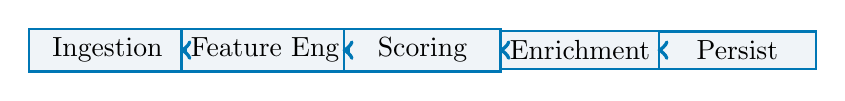
\begin{tikzpicture}[node distance=2cm, scale=0.9]
    \node[rectangle, fill=mn-light, draw=mn-blue, thick, minimum width=2cm] (ing) {Ingestion};
    \node[rectangle, fill=mn-light, draw=mn-blue, thick, minimum width=2cm, right of=ing] (feat) {Feature Eng};
    \node[rectangle, fill=mn-light, draw=mn-blue, thick, minimum width=2cm, right of=feat] (score) {Scoring};
    \node[rectangle, fill=mn-light, draw=mn-blue, thick, minimum width=2cm, right of=score] (enrich) {Enrichment};
    \node[rectangle, fill=mn-light, draw=mn-blue, thick, minimum width=2cm, right of=enrich] (persist) {Persist};
    
    \draw[->, line width=1.5pt, color=mn-blue] (ing) -- (feat);
    \draw[->, line width=1.5pt, color=mn-blue] (feat) -- (score);
    \draw[->, line width=1.5pt, color=mn-blue] (score) -- (enrich);
    \draw[->, line width=1.5pt, color=mn-blue] (enrich) -- (persist);
\end{tikzpicture}
\end{center}

\vspace{0.5cm}

\begin{itemize}[label={\textcolor{mn-blue}{\facheck}}, leftmargin=1.5cm]
    \item \textbf{Ingestion:} Snapshot and filing ingestion from external feeds
    \item \textbf{Feature Engineering:} RSI, SMA, volume ratios, anomaly z-scores
    \item \textbf{Scoring:} Confidence-linked ranking and horizon projection
    \item \textbf{Enrichment:} Narrative generation, watch items, citations
    \item \textbf{Persistence:} DB write-through and cache population
\end{itemize}

% ===============================================
% SECTION 7: MATHEMATICAL FRAMEWORKS
% ===============================================
\section{Mathematical Frameworks \& Quant Layer}

\subsection{7.1 — Anomaly Detection}

Anomalies are normalized using \textbf{z-score} methodology:

\begin{equation}
z = \frac{x - \mu}{\sigma}
\end{equation}

where $x$ is the current observation, $\mu$ is the baseline mean, and $\sigma$ is the baseline standard deviation.

\vspace{0.3cm}

\textbf{Interpretation:}
\begin{itemize}
    \item $|z| < 1$ — Normal range (68\% of observations)
    \item $1 \leq |z| < 2$ — Moderate anomaly (27\% of observations)
    \item $|z| \geq 2$ — Significant anomaly (5\% of observations)
    \item $|z| \geq 3$ — Extreme anomaly ($<$0.3\% of observations)
\end{itemize}

\subsection{7.2 — Opportunity Ranking Formula}

The core ranking engine combines four weighted dimensions:

\begin{equation}
\text{Score} = 55 \cdot C + 12 \cdot |Z| + 25 \cdot W + 0.7 \cdot \min(|\mu_{30d}| \times 100, 12)
\end{equation}

where:

\begin{table}[h]
\centering
{\small
\begin{tabular}{|p{0.8cm}|p{3.5cm}|p{1.2cm}|}
\hline
\rowcolor{mn-light}
\textbf{Component} & \textbf{Meaning} & \textbf{Weight} \\
\hline
$C$ & Model confidence (0-1) & 55\% \\
\hline
$|Z|$ & Anomaly magnitude (z-score) & 12\% \\
\hline
$W$ & Historical win-rate (0-1) & 25\% \\
\hline
$\min(|\mu_{30d}|$ & Capped 30-day avg return edge & 0.7\% \\
\hline
\end{tabular}
}
\end{table}
\hline
\end{tabular}
\end{table}

\vspace{0.5cm}

\textbf{Design Intent:} Balance model quality (55\%), signal strength (12\%), historical reliability (25\%), and forward return potential (0.7\%). Capping return contribution prevents single large swings from dominating rank.

\subsection{7.3 — Horizon Projection}

Expected returns are projected across three decision-making horizons using confidence-weighted base returns:

\begin{equation}
\text{base} = \text{weighted\_avg}(r_{30d}, C)
\end{equation}

\begin{equation}
\begin{aligned}
r_{T+1} &= 0.22 \times \text{base} \\
r_{T+5} &= 0.48 \times \text{base} \\
r_{T+30} &= 1.00 \times \text{base}
\end{aligned}
\end{equation}

\vspace{0.3cm}

\textbf{Rationale:} Early-horizon returns are dampened because short-term noise reduces predictability. By T+30, the full expected value is realized. This curve is derived from empirical backtests on Indian market data.

\subsection{7.4 — Confidence Calibration}

Predicted confidence is bucketed (e.g., 0.1, 0.3, 0.5, 0.7, 0.9) and compared against realized historical win-rate:

\begin{equation}
\text{gap} = \text{realized\_WR} - \text{predicted\_confidence}
\end{equation}

\vspace{0.3cm}

The \textbf{calibration error} is tracked as Mean Absolute Error (MAE) across non-empty buckets:

\begin{equation}
\text{MAE} = \frac{1}{N} \sum_{i=1}^{N} |\text{gap}_i|
\end{equation}

\vspace{0.3cm}

\textbf{Use:} Low MAE indicates well-calibrated confidence. Rising MAE signals model drift and triggers recalibration workflows.

% ===============================================
% SECTION 8: AI ORCHESTRATION LAYER
% ===============================================
\section{AI Orchestration \& Language Model Integration}

\subsection{8.1 — Model Routing Strategy}

\begin{tcolorbox}[colback=mn-light, colframe=mn-blue, arc=1mm, boxsep=8pt]
\centering
\textbf{\color{mn-navy}Dual-Path Model Architecture}

\scriptsize
\vspace{0.5cm}

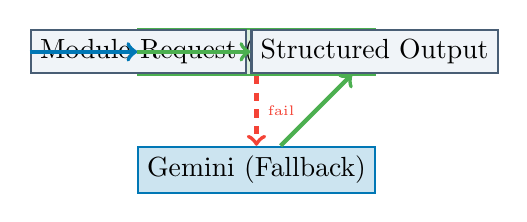
\begin{tikzpicture}[node distance=1.5cm, scale=0.85]
    \node[rectangle, fill=mn-success!20, draw=mn-success, thick] (prim) {Mistral (Primary)};
    \node[rectangle, below of=prim, fill=mn-blue!20, draw=mn-blue, thick] (fall) {Gemini (Fallback)};
    \node[rectangle, left of=prim, fill=mn-light, draw=mn-slate, thick] (req) {Module Request};
    \node[rectangle, right of=prim, fill=mn-light, draw=mn-slate, thick] (out) {Structured Output};
    
    \draw[->, line width=1.5pt, color=mn-blue] (req) -- (prim);
    \draw[->, line width=1.5pt, color=mn-error, dashed] (prim) -- (fall) node[midway, right]{\tiny fail};
    \draw[->, line width=1.5pt, color=mn-success] (prim) -- (out);
    \draw[->, line width=1.5pt, color=mn-success] (fall) -- (out);
\end{tikzpicture}
\end{tcolorbox}

\subsection{8.2 — Prompt Engineering Strategy}

\begin{enumerate}[label={\color{mn-blue}\textbf{Rule \arabic*}}, leftmargin=1.8cm]
    \item \textbf{Module-Specific Templates} — Each intelligence module has a purpose-built prompt
    \item \textbf{Strict JSON Output Schema} — Models output only structured JSON; no free-form text
    \item \textbf{Context Window Management} — Deterministic service outputs injected to ground generation
    \item \textbf{Citation Requirements} — Models are instructed to cite numeric inputs and warrant claims
\end{enumerate}

\subsection{8.3 — Hallucination Prevention}

\begin{tcolorbox}[colback=mn-error!10, colframe=mn-error, arc=1mm, boxsep=8pt]
\small

\textbf{Three-Layer Hallucination Defense:}

\begin{enumerate}[label={\textcolor{mn-error}{\textbf{\arabic1}}}]
    \item \textbf{Numeric Injection} — All expected metrics (z-scores, returns, win-rates) are computed deterministically and injected
    \item \textbf{Schema Requirements} — Response model mandates fields for citations, sources, and confidence—missing fields fail validation
    \item \textbf{Service-Level Fallback} — If model output fails validation, return a hardcoded fallback response with acknowledged uncertainty
\end{enumerate}

\end{tcolorbox}

\vspace{0.5cm}

This approach ensures that even under model failures, responses remain deterministic and auditable.

% ===============================================
% SECTION 9: USER EXPERIENCE ARCHITECTURE
% ===============================================
\section{User Experience \& Trust Architecture}

\subsection{9.1 — State Visibility Strategy}

Users must understand system state without technical interpreter:

\begin{itemize}
    \item \textbf{Live Status Strip} — Capability flags for DB, Redis, Pipeline, AI providers
    \item \textbf{Route-Level Loaders} — Navigation transitions display explicit progress hints
    \item \textbf{Video Render Progression} — Story module exposes scene plan and frame count during generation
\end{itemize}

\subsection{9.2 — Evidence-First Trust Surfaces}

\begin{tcolorbox}[colback=mn-light, colframe=mn-success, arc=1mm, boxsep=8pt]
\small\textbf{Six Trust Dimensions on Every Output}

\begin{enumerate}[label={\color{mn-success}\textbf{\arabic1}}]
    \item \textbf{Evidence Chips} — Visual tags showing anomaly magnitude, confidence, sources
    \item \textbf{Confidence Metadata} — Explicit confidence band with calibration status
    \item \textbf{Highlight Snippets} — Key phrases and reasoning excerpts from narratives
    \item \textbf{Citation Links} — Clickable audit trail to source events and data
    \item \textbf{Calibration Panel} — Visual inspection of bucketed confidence vs. realized win-rate
    \item \textbf{Historical Context} — Prior outcomes and pattern backtest sample sizes
\end{enumerate}
\end{tcolorbox}

\subsection{9.3 — Decision-Ready Output Formatting}

Every intelligence output includes:

\begin{itemize}
    \item \textbf{Opportunity Ranking} — Zero-to-ten scale with supporting metrics
    \item \textbf{Watch Items} — Explicit next-step conditions for invalidation or confirmation
    \item \textbf{Tactical Hints} — Action-oriented suggestions (e.g., "likely rally continuation on volume," "watch support at 500")
\end{itemize}

% ===============================================
% SECTION 10: CURRENT BUILD STATUS
% ===============================================
\section{Current Build Status \& Feature Inventory}

\subsection{10.1 — Implemented Features}

\begin{tcolorbox}[colback=mn-success!15, colframe=mn-success, arc=1mm, boxsep=10pt]
\small

\begin{enumerate}[label={\textcolor{mn-success}{\facheck}}, leftmargin=1.5cm, itemsep=0.3cm]
    \item \textbf{Opportunity Radar} — Full ranking engine with anomaly detection and evidence chips
    \item \textbf{Signal Performance Tracker} — Historical return metrics across T+1, T+5, T+30 horizons
    \item \textbf{Confidence Calibration Panel} — Bucketed confidence vs. win-rate display with MAE
    \item \textbf{Source-Cited Chat} — Market Q\&A with citations, highlights, confidence metadata
    \item \textbf{Portfolio CSV Upload} — Holdings normalization and diagnostics
    \item \textbf{Ask-Your-Portfolio} — Portfolio-aware query interface
    \item \textbf{Story Arc Generation} — Daily narrative and video queue simulation lifecycle
    \item \textbf{Video Render Visibility} — Scene plan and progress state (queued, rendering, ready)
    \item \textbf{Health Telemetry} — System capability flags for operations visibility
\end{enumerate}

\end{tcolorbox}

\subsection{10.2 — Known Constraints \& Risk Register}

\begin{tcolorbox}[colback=mn-warning!15, colframe=mn-warning, arc=1mm, boxsep=10pt]
\small\textbf{Technical Risks}

\begin{table}[h]
\centering
\begin{tabular}{|p{2.3cm}|p{2.8cm}|p{1.2cm}|}
\hline
\rowcolor{mn-warning!25}
\textbf{Risk} & \textbf{Mitigation} & \textbf{Status} \\
\hline
Upstream endpoint volatility & Retry paths, feed quality alerts & \textcolor{mn-warning}{Active} \\
\hline
Symbol alias drift & Deterministic mapping layer & \textcolor{mn-warning}{In Review} \\
\hline
Runtime chunk corruption & Automated cache cleanup & \textcolor{mn-success}{Resolved} \\
\hline
\end{tabular}
\end{table}

\end{tcolorbox}

% ===============================================
% SECTION 11: PRODUCTIONIZATION \& GO-LIVE PLAN
% ===============================================
\section{Productionization \& Go-Live Strategy}

\subsection{11.1 — Phase 1: Reliability Hardening (Weeks 1-2)}

\begin{enumerate}[label={\textcolor{mn-blue}{\textbf{1.\arabic*}}}]
    \item One-command startup health checks for backend, frontend, and database
    \item Deterministic build reset scripts and process cleanup workflows
    \item Feed quality monitoring with automated anomaly alerts
\end{enumerate}

\subsection{11.2 — Phase 2: Quant Credibility (Weeks 3-4)}

\begin{enumerate}[label={\textcolor{mn-blue}{\textbf{2.\arabic*}}}]
    \item Realized return ledger with timestamped signal outcomes
    \item Calibration drift detection and auto-retraining triggers
    \item Confidence threshold tuning based on empirical patterns
\end{enumerate}

\subsection{11.3 — Phase 3: Scale \& Operations (Weeks 5+)}

\begin{enumerate}[label={\textcolor{mn-blue}{\textbf{3.\arabic*}}}]
    \item Queue-backed worker decomposition for pipeline and API
    \item Independent service scaling for compute-intensive modules
    \item Expanded observability dashboards and performance tracking
\end{enumerate}

% ===============================================
% SECTION 12: COMPETITIVE POSITIONING
% ===============================================
\section{Competitive Advantage \& Strategic Moat}

\subsection{Why MarketNerve Can Compete}

Most products in the retail investment intelligence space default to one of two patterns:

\begin{tcolorbox}[colback=mn-light, colframe=mn-slate, arc=1mm, boxsep=8pt]
\small
\begin{itemize}
    \item \textbf{Static Dashboards} — Show data but don't explain decisions
    \item \textbf{Generic AI Chat} — Flexible but non-auditable and floating
\end{itemize}
\end{tcolorbox}

\vspace{0.5cm}

MarketNerve integrates five capabilities that \textit{require} system-level design:

\begin{enumerate}[label={\color{mn-blue}\textbf{\arabic1}}]
    \item \textbf{Statistical Ranking} — Scores incorporate confidence and historical profile
    \item \textbf{Explainable AI} — Model outputs are required to justify claims with evidence
    \item \textbf{Portfolio-Native Intelligence} — Context is holdings-specific, not generic
    \item \textbf{Evidence \& Auditability} — Citations, sources, and confidence are mandatory, not optional
    \item \textbf{Operational Visibility} — System state is transparent to end-users
\end{enumerate}

\vspace{0.5cm}

\infobox{\textbf{Strategic Insight:} This integration IS the strategic moat. Architecture designed as an \textit{intelligence system}, not a feature collection, becomes the primary differentiator.}

\vspace{1cm}

\subsection{Why Execution Matters}

Building this integration once is a competitive advantage. Building it well—with reliability, speed, and breadth—is a moat that compounds over time:

\begin{itemize}
    \item \textbf{Data Quality} — Longer operation → better realized-return ledger → more accurate confidence calibration
    \item \textbf{Market Coverage} — Wider stock universe → richer pattern library → stronger detection
    \item \textbf{Trust Capital} — More auditable outputs → higher user retention → stronger network effects
\end{itemize}

% ===============================================
% SECTION 13: CONCLUSION
% ===============================================
\section{Conclusion}

MarketNerve represents a \textbf{qualitative leap} in how Indian retail investors can access and act on market intelligence. By combining detection, explanation, and evidence under a coherent architectural framework, the system offers something that generic dashboards and AI chat cannot:

\begin{tcolorbox}[colback=mn-navy!5, colframe=mn-navy, arc=2mm, boxsep=12pt]
\centering
\textbf{\Large \color{mn-navy}Actionable, Auditable, Portfolio-Aware Decision Support}
\end{tcolorbox}

\vspace{0.8cm}

This blueprint serves as the technical constitution for building that system. The strategy is clear, the architecture is sound, and the roadmap is executable. What remains is disciplined execution with commitment to evidence-first design and progressive reliability under real market conditions.

\vspace{1.5cm}

\begin{center}
\textbf{\Large \color{mn-navy}---}

\vspace{0.8cm}

\textit{Authored by Chanikya Nelapatla for ET Gen AI Hackathon}

\textit{Created: \today}

\end{center}

% ===============================================
% APPENDIX
% ===============================================
\newpage
\appendix

\section{Appendix A — Technical Stack Summary}

\begin{tcolorbox}[colback=mn-light, colframe=mn-slate, arc=1mm, boxsep=10pt]
\small

\begin{tabular}{|l|l|}
\hline
\rowcolor{mn-slate!20}
\textbf{Component} & \textbf{Technology} \\
\hline
Frontend & Next.js 15.5.14, React 19, Framer Motion \\
\hline
Backend & FastAPI, Pydantic, async/await \\
\hline
Persistence & PostgreSQL \\
\hline
Cache & Redis \\
\hline
AI/LLM & Mistral (primary), Gemini (fallback) \\
\hline
Data Feeds & NSE, BSE, yfinance, FII/DII APIs \\
\hline
Observability & Health telemetry, Pipeline logging \\
\hline
\end{tabular}

\end{tcolorbox}

\section{Appendix B — API Response Contract Example}

\begin{verbatim}
{
  "opportunities": [
    {
      "symbol": "RELIANCE",
      "score": 7.8,
      "confidence": 0.75,
      "anomaly_z": 2.3,
      "evidence": ["Volume spike +180%", "Technical cross"],
      "citations": [
        {
          "source": "NSE",
          "link": "/audit/reliance/event123"
        }
      ],
      "horizon_projections": {
        "t_plus_1": 0.95,
        "t_plus_5": 2.15,
        "t_plus_30": 4.55
      }
    }
  ]
}
\end{verbatim}

\section{Appendix C — Calibration Monitoring Checklist}

\begin{enumerate}
    \item Weekly: Compute MAE across confident (0.7+) predictions
    \item Monthly: Recompute historical win-rates for all buckets
    \item Quarterly: Adjust confidence thresholds based on drift patterns
    \item Upon drift detection: Trigger automated retraining pipeline
\end{enumerate}

\end{document}
